\section{Thảo luận và mở rộng}
Qua việc tim hiểu và phân tích mô hình hôi quy tuyến tính bằng ngôn ngữ R, dựa trên những cơ sở lý thuyết đã học và tìm hiểu thêm nhóm chúng tôi đã biết thêm về các phương thức xử lý các số liệu gốc và mô hình hóa nó để phục vụ mục đích tim hiểu và phân tích dữ liệu. Từ đó có thể áp dụng thực hiện đối với các dữ liệu trong thực tế. Tuy nhiên qua việc làm việc với mô hình hôi quy chúng tôi rút ra nhận xét mô hình hồi quy tuyến tính có những ưu điểm và khuyết điểm sau:

Ưu điểm:
\begin{itemize}
    \item Nhanh chóng để mô hình hóa và đặc biệt hữu ích khi mối quan hệ được mô hình hóa không quá phức tạp và nếu bạn không có nhiều dữ liệu.
    \item Hồi quy tuyến tính là đơn giản để hiểu
\end{itemize}

Khuyết điểm:
\begin{itemize}
    \item Nhạy cảm với dữ liệu nhiễu.
    \item Không biểu diễn được những mô hình phức tạp
\end{itemize}

Ngoài ra, nhóm đề xuất nghiên cứu thêm mô hình hồi quy logistic. Do nguồn lực có hạn, chúng tôi sẽ trình bày vắn tắt kết quả vận dụng mô hình này để xác định xác suất hài lòng của khách hàng (\textbf{is\_happy\_customer}) dựa trên kho hàng gần nhất (\textbf{nearest\_warehouse}).

Hình \ref{fig:6.1} cho thấy với mỗi nơi cung ứng sản phẩm, lượng khách hàng hài lòng luôn chiếm ưu thế.
\begin{figure}[!htbp]
    \centering
    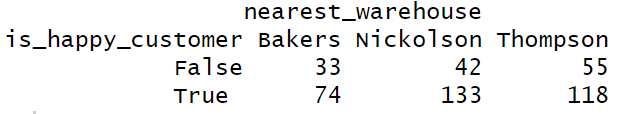
\includegraphics[width=0.5\textwidth]{graphics/mo_rong/f1.PNG}
    \caption{Bảng dữ liệu của \textbf{is\_happy\_customer} và \textbf{nearest\_warehouse}}
    \label{fig:6.1} 
\end{figure}

Để vận dụng mô hình trên, ta sẽ sử dụng hàm \textbf{glm} với đầu vào \textbf{is\_happy\_customer \textasciitilde .}, nghĩa là \textbf{is\_happy\_customer} sẽ phụ thuộc vào các biến còn lại trong \textbf{df}. Lưu ý cần phải chỉ định \textbf{family = "binomial"} để mô hình hoạt động đúng theo hồi quy logistic. Kết quả được thể hiện trên hình \ref{fig:logistic}
\begin{figure}[!htbp]
    \centering
    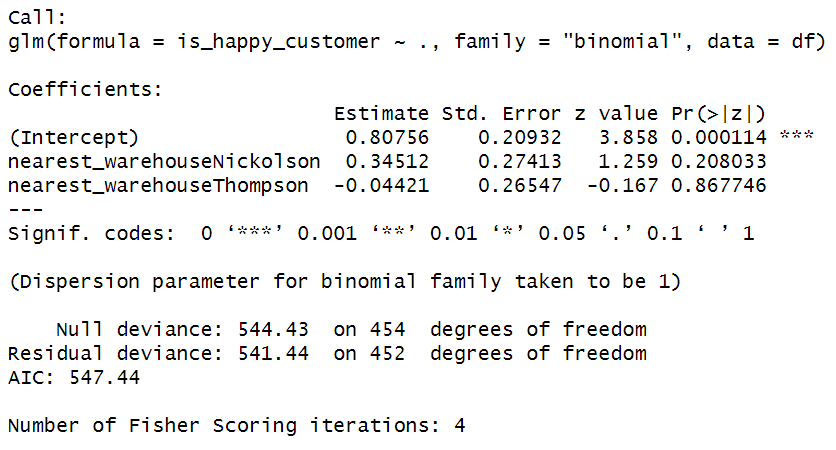
\includegraphics[width=0.6\textwidth]{graphics/mo_rong/f2.PNG}
    \caption{Kết quả của mô hình hồi quy logistic}
    \label{fig:logistic}
\end{figure}

Ta chỉ xét kho hàng có ý nghĩa thống kê chính là kho Bakers với P-value=0.000114 (<5\%). Hệ số được ước lượng gọi là log odds và bằng 0.80756. Dựa vào giá trị đó, ta dự đoán được xác suất hài lòng của khách hàng khi mua tại kho hàng Bakers theo công thức sau:
\[
    P(Y=1|X=\text{Bakers}) = \frac{1}{1 + e^{-0.80756}} = 0.6916
\]
Như vậy, 69.16\% khả năng khách hàng sẽ hài lòng nếu mua hàng tại kho hàng Bakers. Nếu áp dụng Threshold=50\% để phân loại kết quả, ta có thể kết luận khách hàng có hài lòng!

Khác với hồi quy tuyến tính đa bội, hồi quy logistic có khả năng xử lý những biến phân loại nhị thức hiệu quả hơn qua việc dự đoán xác suất trong khoảng từ 0 đến 1. Nó sử dụng phương pháp \textbf{Maximum likelihood estimation} trong khi hồi quy tuyến tính đa bội sử dụng \textbf{Least squares}.